\subsubsection{General Approach}

The chess commentator has the task to convert certain information, which it receives from the chess engine described before, into human understandable comments. Such a task falls into the domain of \textit{sequence-to-sequence} processing. The idea of sequence-to-sequence models are that an input of a certain length is mapped to an output of a certain length, where input and output length can be different. For such tasks, encoder-decoder architectures with attention has achieved great success in the past. The architecture consists of two parts, an encoder and a decoder, which are two \textit{bidirectional recurrent neural networks (BRNN) using long short-term memory (LSTM) state cells}.

Recurrent neural networks (RNN) are a special type of neural network designed to process sequential inputs and recognize patterns in them. Due to an internal memory, RNNs are able to remember and reuse certain characteristics of the input. In general, an RNN works as follows: (1) recive an input (2) let the neurons generate an output, (3) copy that output (4) take the copied output and the new input and return to (1). Thus, the new RNN input consists of the output generated in the past and the new sequence part added, allowing the network to build a deep understanding of the sequence. An extension of an recurrent neural networks are bidirectional recurrent neural networks. While the neurons of RNNs always pass the generated output to the neuron in the immediate future, in BRNNs there is another level of neurons that can pass the output to past neurons. By including information from both the past and the future, an even deeper understanding of the sequence can be built. When \cite{Sutskever-2014-sts} first introducted their sequence to sequence model they used RNN with long short-term memory state cells. Those are a special neuronal architecture of an RNN, which is why it is also simply referred to as LSTM or BLSTM (in case of bidirectional LSTMs). LSTM use a special kind of neurons, called state cells, which solve problems of RNNs and BRNNs that make it difficult to train them.

The encoder-decoder architecture used for generating chess comments makes use of the described BLSTMs. The idea of the architecture is that the encoder receives a sequence of data step by step, processes the data and encodes it into a fixed length vector. This vector are the last states of the encoder, used by the decoder to set its initial states to it to produce the desired translation. One problem that affects the quality of the decoder's translation, is the length of the sequences. The sequence stored in the vector tends to dilute over time, resulting in poor translations. To solve it, an attention mechanisms can be used. When processing the data, only the most important information received is considered, so the vector, called the context vector, contains only a summary of the sequence. This allows the decoder to focus only on the information relevant for translation. If the decoder now wants to generate comments, it receives a start symbol as input (represented by \texttt{<START>} in Figure \ref{fig:eda}). This start symbol is used to indicate the start of the output sequence. The first output is the first word of the translation. The output is additionally used as new input in the next step, generates an output and which is used as the new input again. This procedure is repeated until an end symbol is reached, which signals the end of the sequence. The generated output sequence is the translation.

\begin{figure}[h]
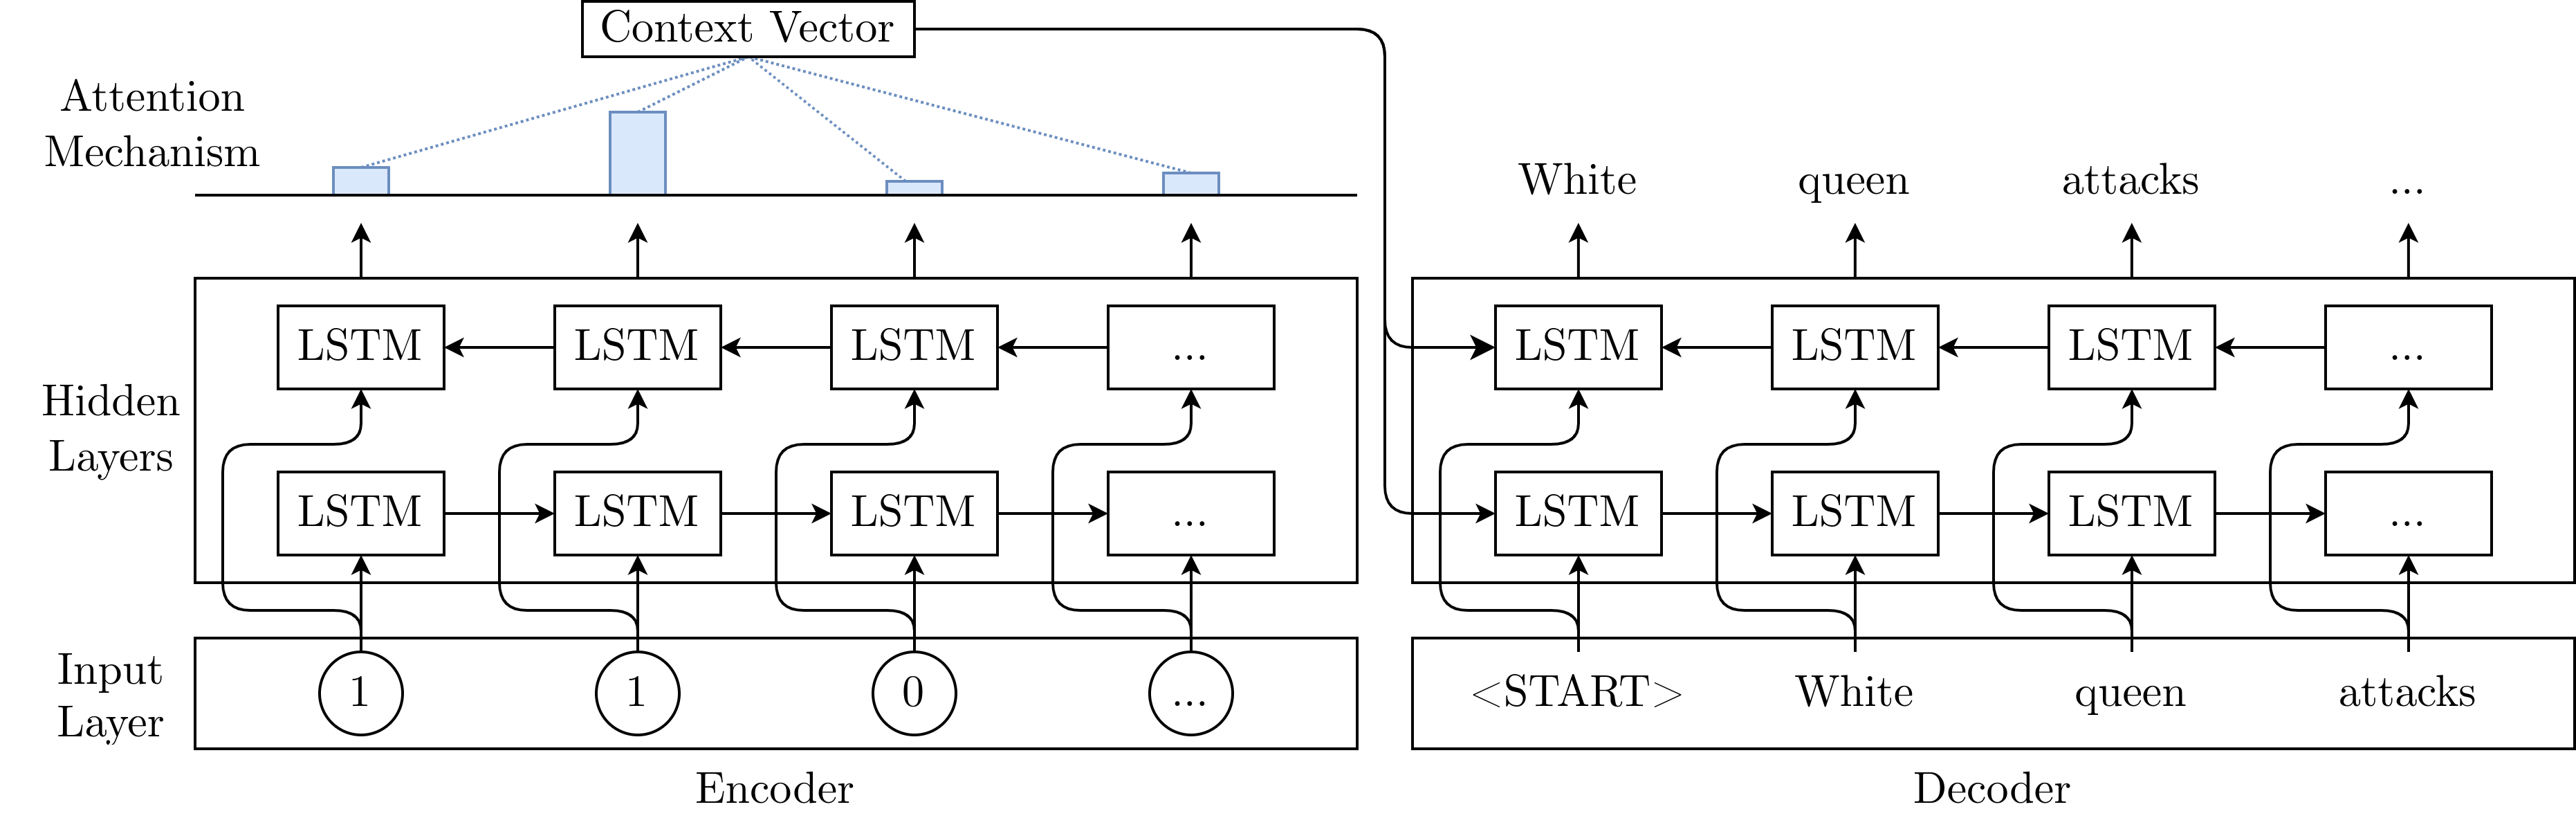
\includegraphics[width=1\textwidth]{graphics/commentator_example/general_approach.png}
\caption{Chess Commentator Encoder-Decoder Architecture with Attention Mechanism}
\label{fig:eda}
\end{figure}